
%% bare_conf_compsoc.tex
%% V1.4b
%% 2015/08/26
%% by Michael Shell
%% See:
%% http://www.michaelshell.org/
%% for current contact information.
%%
%% This is a skeleton file demonstrating the use of IEEEtran.cls
%% (requires IEEEtran.cls version 1.8b or later) with an IEEE Computer
%% Society conference paper.
%%
%% Support sites:
%% http://www.michaelshell.org/tex/ieeetran/
%% http://www.ctan.org/pkg/ieeetran
%% and
%% http://www.ieee.org/

%%*************************************************************************
%% Legal Notice:
%% This code is offered as-is without any warranty either expressed or
%% implied; without even the implied warranty of MERCHANTABILITY or
%% FITNESS FOR A PARTICULAR PURPOSE! 
%% User assumes all risk.
%% In no event shall the IEEE or any contributor to this code be liable for
%% any damages or losses, including, but not limited to, incidental,
%% consequential, or any other damages, resulting from the use or misuse
%% of any information contained here.
%%
%% All comments are the opinions of their respective authors and are not
%% necessarily endorsed by the IEEE.
%%
%% This work is distributed under the LaTeX Project Public License (LPPL)
%% ( http://www.latex-project.org/ ) version 1.3, and may be freely used,
%% distributed and modified. A copy of the LPPL, version 1.3, is included
%% in the base LaTeX documentation of all distributions of LaTeX released
%% 2003/12/01 or later.
%% Retain all contribution notices and credits.
%% ** Modified files should be clearly indicated as such, including  **
%% ** renaming them and changing author support contact information. **
%%*************************************************************************


% *** Authors should verify (and, if needed, correct) their LaTeX system  ***
% *** with the testflow diagnostic prior to trusting their LaTeX platform ***
% *** with production work. The IEEE's font choices and paper sizes can   ***
% *** trigger bugs that do not appear when using other class files.       ***                          ***
% The testflow support page is at:
% http://www.michaelshell.org/tex/testflow/



\documentclass[conference]{IEEEtran}

% Uncomment \blindtrue for double-blind review
\newif\ifblind
\blindtrue

% Some/most Computer Society conferences require the compsoc mode option,
% but others may want the standard conference format.
%
% If IEEEtran.cls has not been installed into the LaTeX system files,
% manually specify the path to it like:
% \documentclass[conference,compsoc]{../sty/IEEEtran}


\usepackage[table]{xcolor}
\usepackage{tikz}
\usetikzlibrary{shapes.geometric}


% Some very useful LaTeX packages include:
% (uncomment the ones you want to load)


% *** MISC UTILITY PACKAGES ***
%
%\usepackage{ifpdf}
% Heiko Oberdiek's ifpdf.sty is very useful if you need conditional
% compilation based on whether the output is pdf or dvi.
% usage:
% \ifpdf
%   % pdf code
% \else
%   % dvi code
% \fi
% The latest version of ifpdf.sty can be obtained from:
% http://www.ctan.org/pkg/ifpdf
% Also, note that IEEEtran.cls V1.7 and later provides a builtin
% \ifCLASSINFOpdf conditional that works the same way.
% When switching from latex to pdflatex and vice-versa, the compiler may
% have to be run twice to clear warning/error messages.






% *** CITATION PACKAGES ***
%
\ifCLASSOPTIONcompsoc
  % IEEE Computer Society needs nocompress option
  % requires cite.sty v4.0 or later (November 2003)
  \usepackage[nocompress]{cite}
\else
  % normal IEEE
  \usepackage{cite}
\fi
% cite.sty was written by Donald Arseneau
% V1.6 and later of IEEEtran pre-defines the format of the cite.sty package
% \cite{} output to follow that of the IEEE. Loading the cite package will
% result in citation numbers being automatically sorted and properly
% "compressed/ranged". e.g., [1], [9], [2], [7], [5], [6] without using
% cite.sty will become [1], [2], [5]--[7], [9] using cite.sty. cite.sty's
% \cite will automatically add leading space, if needed. Use cite.sty's
% noadjust option (cite.sty V3.8 and later) if you want to turn this off
% such as if a citation ever needs to be enclosed in parenthesis.
% cite.sty is already installed on most LaTeX systems. Be sure and use
% version 5.0 (2009-03-20) and later if using hyperref.sty.
% The latest version can be obtained at:
% http://www.ctan.org/pkg/cite
% The documentation is contained in the cite.sty file itself.
%
% Note that some packages require special options to format as the Computer
% Society requires. In particular, Computer Society  papers do not use
% compressed citation ranges as is done in typical IEEE papers
% (e.g., [1]-[4]). Instead, they list every citation separately in order
% (e.g., [1], [2], [3], [4]). To get the latter we need to load the cite
% package with the nocompress option which is supported by cite.sty v4.0
% and later.





% *** GRAPHICS RELATED PACKAGES ***
%
\ifCLASSINFOpdf
  % \usepackage[pdftex]{graphicx}
  % declare the path(s) where your graphic files are
  % \graphicspath{{../pdf/}{../jpeg/}}
  % and their extensions so you won't have to specify these with
  % every instance of \includegraphics
  % \DeclareGraphicsExtensions{.pdf,.jpeg,.png}
\else
  % or other class option (dvipsone, dvipdf, if not using dvips). graphicx
  % will default to the driver specified in the system graphics.cfg if no
  % driver is specified.
  % \usepackage[dvips]{graphicx}
  % declare the path(s) where your graphic files are
  % \graphicspath{{../eps/}}
  % and their extensions so you won't have to specify these with
  % every instance of \includegraphics
  % \DeclareGraphicsExtensions{.eps}
\fi
% graphicx was written by David Carlisle and Sebastian Rahtz. It is
% required if you want graphics, photos, etc. graphicx.sty is already
% installed on most LaTeX systems. The latest version and documentation
% can be obtained at: 
% http://www.ctan.org/pkg/graphicx
% Another good source of documentation is "Using Imported Graphics in
% LaTeX2e" by Keith Reckdahl which can be found at:
% http://www.ctan.org/pkg/epslatex
%
% latex, and pdflatex in dvi mode, support graphics in encapsulated
% postscript (.eps) format. pdflatex in pdf mode supports graphics
% in .pdf, .jpeg, .png and .mps (metapost) formats. Users should ensure
% that all non-photo figures use a vector format (.eps, .pdf, .mps) and
% not a bitmapped formats (.jpeg, .png). The IEEE frowns on bitmapped formats
% which can result in "jaggedy"/blurry rendering of lines and letters as
% well as large increases in file sizes.
%
% You can find documentation about the pdfTeX application at:
% http://www.tug.org/applications/pdftex





% *** MATH PACKAGES ***
%
%\usepackage{amsmath}
% A popular package from the American Mathematical Society that provides
% many useful and powerful commands for dealing with mathematics.
%
% Note that the amsmath package sets \interdisplaylinepenalty to 10000
% thus preventing page breaks from occurring within multiline equations. Use:
%\interdisplaylinepenalty=2500
% after loading amsmath to restore such page breaks as IEEEtran.cls normally
% does. amsmath.sty is already installed on most LaTeX systems. The latest
% version and documentation can be obtained at:
% http://www.ctan.org/pkg/amsmath





% *** SPECIALIZED LIST PACKAGES ***
%
%\usepackage{algorithmic}
% algorithmic.sty was written by Peter Williams and Rogerio Brito.
% This package provides an algorithmic environment fo describing algorithms.
% You can use the algorithmic environment in-text or within a figure
% environment to provide for a floating algorithm. Do NOT use the algorithm
% floating environment provided by algorithm.sty (by the same authors) or
% algorithm2e.sty (by Christophe Fiorio) as the IEEE does not use dedicated
% algorithm float types and packages that provide these will not provide
% correct IEEE style captions. The latest version and documentation of
% algorithmic.sty can be obtained at:
% http://www.ctan.org/pkg/algorithms
% Also of interest may be the (relatively newer and more customizable)
% algorithmicx.sty package by Szasz Janos:
% http://www.ctan.org/pkg/algorithmicx




% *** ALIGNMENT PACKAGES ***
%
%\usepackage{array}
% Frank Mittelbach's and David Carlisle's array.sty patches and improves
% the standard LaTeX2e array and tabular environments to provide better
% appearance and additional user controls. As the default LaTeX2e table
% generation code is lacking to the point of almost being broken with
% respect to the quality of the end results, all users are strongly
% advised to use an enhanced (at the very least that provided by array.sty)
% set of table tools. array.sty is already installed on most systems. The
% latest version and documentation can be obtained at:
% http://www.ctan.org/pkg/array


% IEEEtran contains the IEEEeqnarray family of commands that can be used to
% generate multiline equations as well as matrices, tables, etc., of high
% quality.




% *** SUBFIGURE PACKAGES ***
\ifCLASSOPTIONcompsoc
  \usepackage[caption=false,font=small,labelfont=sf,textfont=sf]{subfig}
\else
  \usepackage[caption=false,font=small]{subfig}
\fi
% subfig.sty, written by Steven Douglas Cochran, is the modern replacement
% for subfigure.sty, the latter of which is no longer maintained and is
% incompatible with some LaTeX packages including fixltx2e. However,
% subfig.sty requires and automatically loads Axel Sommerfeldt's caption.sty
% which will override IEEEtran.cls' handling of captions and this will result
% in non-IEEE style figure/table captions. To prevent this problem, be sure
% and invoke subfig.sty's "caption=false" package option (available since
% subfig.sty version 1.3, 2005/06/28) as this is will preserve IEEEtran.cls
% handling of captions.
% Note that the Computer Society format requires a sans serif font rather
% than the serif font used in traditional IEEE formatting and thus the need
% to invoke different subfig.sty package options depending on whether
% compsoc mode has been enabled.
%
% The latest version and documentation of subfig.sty can be obtained at:
% http://www.ctan.org/pkg/subfig




% *** FLOAT PACKAGES ***
%
%\usepackage{fixltx2e}
% fixltx2e, the successor to the earlier fix2col.sty, was written by
% Frank Mittelbach and David Carlisle. This package corrects a few problems
% in the LaTeX2e kernel, the most notable of which is that in current
% LaTeX2e releases, the ordering of single and double column floats is not
% guaranteed to be preserved. Thus, an unpatched LaTeX2e can allow a
% single column figure to be placed prior to an earlier double column
% figure.
% Be aware that LaTeX2e kernels dated 2015 and later have fixltx2e.sty's
% corrections already built into the system in which case a warning will
% be issued if an attempt is made to load fixltx2e.sty as it is no longer
% needed.
% The latest version and documentation can be found at:
% http://www.ctan.org/pkg/fixltx2e


%\usepackage{stfloats}
% stfloats.sty was written by Sigitas Tolusis. This package gives LaTeX2e
% the ability to do double column floats at the bottom of the page as well
% as the top. (e.g., "\begin{figure*}[!b]" is not normally possible in
% LaTeX2e). It also provides a command:
%\fnbelowfloat
% to enable the placement of footnotes below bottom floats (the standard
% LaTeX2e kernel puts them above bottom floats). This is an invasive package
% which rewrites many portions of the LaTeX2e float routines. It may not work
% with other packages that modify the LaTeX2e float routines. The latest
% version and documentation can be obtained at:
% http://www.ctan.org/pkg/stfloats
% Do not use the stfloats baselinefloat ability as the IEEE does not allow
% \baselineskip to stretch. Authors submitting work to the IEEE should note
% that the IEEE rarely uses double column equations and that authors should try
% to avoid such use. Do not be tempted to use the cuted.sty or midfloat.sty
% packages (also by Sigitas Tolusis) as the IEEE does not format its papers in
% such ways.
% Do not attempt to use stfloats with fixltx2e as they are incompatible.
% Instead, use Morten Hogholm'a dblfloatfix which combines the features
% of both fixltx2e and stfloats:
%
% \usepackage{dblfloatfix}
% The latest version can be found at:
% http://www.ctan.org/pkg/dblfloatfix




% *** PDF, URL AND HYPERLINK PACKAGES ***
%
%\usepackage{url}
% url.sty was written by Donald Arseneau. It provides better support for
% handling and breaking URLs. url.sty is already installed on most LaTeX
% systems. The latest version and documentation can be obtained at:
% http://www.ctan.org/pkg/url
% Basically, \url{my_url_here}.




% *** Do not adjust lengths that control margins, column widths, etc. ***
% *** Do not use packages that alter fonts (such as pslatex).         ***
% There should be no need to do such things with IEEEtran.cls V1.6 and later.
% (Unless specifically asked to do so by the journal or conference you plan
% to submit to, of course. )


% correct bad hyphenation here
\hyphenation{DornerWorks pri-ma-ry}


\begin{document}
%
% paper title
% Titles are generally capitalized except for words such as a, an, and, as,
% at, but, by, for, in, nor, of, on, or, the, to and up, which are usually
% not capitalized unless they are the first or last word of the title.
% Linebreaks \\ can be used within to get better formatting as desired.
% Do not put math or special symbols in the title.
\title{Improving ARINC 653 System Reliability by\\Using Fault-Tolerant Partition Scheduling}


% author names and affiliations
% use a multiple column layout for up to three different
% affiliations
\ifblind
\else
\author{\IEEEauthorblockN{Aufar Gilbran}
	\IEEEauthorblockA{School of Electrical Engineering\\and Informatics\\
		Institut Teknologi Bandung\\
		Bandung, Indonesia\\
	Email: aufargilbran@gmail.com}
	\and
	\IEEEauthorblockN{Achmad Imam Kistijantoro}
	\IEEEauthorblockA{School of Electrical Engineering\\and Informatics\\
		Institut Teknologi Bandung\\
		Bandung, Indonesia\\
Email: imam@stei.itb.ac.id}}
\fi

% conference papers do not typically use \thanks and this command
% is locked out in conference mode. If really needed, such as for
% the acknowledgment of grants, issue a \IEEEoverridecommandlockouts
% after \documentclass

% for over three affiliations, or if they all won't fit within the width
% of the page (and note that there is less available width in this regard for
% compsoc conferences compared to traditional conferences), use this
% alternative format:
% 
%\author{\IEEEauthorblockN{Michael Shell\IEEEauthorrefmark{1},
%Homer Simpson\IEEEauthorrefmark{2},
%James Kirk\IEEEauthorrefmark{3}, 
%Montgomery Scott\IEEEauthorrefmark{3} and
%Eldon Tyrell\IEEEauthorrefmark{4}}
%\IEEEauthorblockA{\IEEEauthorrefmark{1}School of Electrical and Computer Engineering\\
%Georgia Institute of Technology,
%Atlanta, Georgia 30332--0250\\ Email: see http://www.michaelshell.org/contact.html}
%\IEEEauthorblockA{\IEEEauthorrefmark{2}Twentieth Century Fox, Springfield, USA\\
%Email: homer@thesimpsons.com}
%\IEEEauthorblockA{\IEEEauthorrefmark{3}Starfleet Academy, San Francisco, California 96678-2391\\
%Telephone: (800) 555--1212, Fax: (888) 555--1212}
%\IEEEauthorblockA{\IEEEauthorrefmark{4}Tyrell Inc., 123 Replicant Street, Los Angeles, California 90210--4321}}




% use for special paper notices
%\IEEEspecialpapernotice{(Invited Paper)}




% make the title area
\maketitle

% As a general rule, do not put math, special symbols or citations
% in the abstract
\begin{abstract}
	The ARINC 653 specifies multiple operating system components to provide isolation
	between partitions. This means failure on one partition does not affect any other
	partition.  While each partition cannot affect the other partitions, the failure still
	happens and possibly leads to failure to the whole system. In this paper, we extend the
	partition scheduler on ARINC 653 compliant hypervisor called ARLX to use primary-backup
	scheme. The resulting scheduler will be able to provide the needed service on failed
	partitions through their backup partitions.
\end{abstract}

\vspace{10pt}

\renewcommand\IEEEkeywordsname{Keywords}
\begin{IEEEkeywords}
	hierarchical, real-time systems, scheduling, reliability, fault-tolerance
\end{IEEEkeywords}

% For peer review papers, you can put extra information on the cover
% page as needed:
% \ifCLASSOPTIONpeerreview
% \begin{center} \bfseries EDICS Category: 3-BBND \end{center}
% \fi
%
% For peerreview papers, this IEEEtran command inserts a page break and
% creates the second title. It will be ignored for other modes.
\IEEEpeerreviewmaketitle



\section{Introduction}
% no \IEEEPARstart
% You must have at least 2 lines in the paragraph with the drop letter
% (should never be an issue)

ARINC 653 is a software specification which primary purpose is to provide isolation or
partitioning of application domains. The specified partitioning scheme in ARINC 653 will prevent
one domain to affect other domains by any means. This could be achieved by making sure each
domain has their own portion of shared resources, including, but not limited to CPU time,
memory, and I/O bandwidth.

Isolation and partitioning is important in aviation \cite{Rushby2000}, as it allows multiple
application each with their own possibly different level of certification to be run in different
partitions on the same platform. An example of such platform is Integrated Modular Avionics
(IMA) systems. These systems were created to supersede federated systems, which maintain
application isolation by having separated platform for each application. ARINC 653 was created
to standardized operating systems for these platforms.

ARINC 653 specification protect each application from the fault that is experienced by other
applications in different partition. Despite being protected of fault from other domains, any
fault the application experienced from its own partition will still happen. It might be the case
that the faulty application or partition is a safety-critical system or part of such system.
Failure of such application or partition leads to a significant increase of the safety risk for
the people and/or partition involved. This leads to the need of system reliability in the
platform or operating system to reduce the safety risk in case of failure.

There are several ways to achieve system reliability in ARINC 653 operating systems. One way is
to make sure the application and its partition would continue to operate even when it has
failed. This could be done by having domains that have the same applications and partition to
replace the faulty domain. These domains are called backup domains and the replaced domain is
called the primary domain. In normal situations, the backup domains will not be given any CPU
time and will reside in background. Once the hypervisor detect that the primary domain
experienced a fault, one of the backup domains will replace it to provide service that is
compatible with the required services. The described scheduling algorithm is called
primary-backup scheduling.

The primary-backup scheduling algorithm is implemented on ARINC 653 compliant hypervisor called
ARLX. The ARLX hypervisor is an ARINC 653 compliant extension to the open-source Xen hypervisor
and is developed by DornerWorks, according to the strict safety assurance directed by DO-178.
It is created to increases the pace of innovation and reduce development of ARINC 653 operating
systems by giving researchers access to working prototype and engineers the freedom of open
source license. Since the ARLX hypervisor already provide ARINC 653 scheduler with ARINC 653
compliant scheduling algorithm, we only need to extend the current ARINC 653 scheduler
scheduling algorithm to support picking between primary and backup domains.

This paper will focus on the implementation of primary-backup scheduling algorithm on ARINC 653
compliant hypervisor. The main topic of this paper includes describing the primary-backup ARINC
653 scheduling algorithm and analysis of the resulting scheduler in different scenarios.

The rest of this paper is organized as follows. In Section II, we will cover the current
implementation of ARINC 653 scheduler in ARLX and primary-backup scheduling algorithm. In
Section III we introduce the proposed primary-backup ARINC 653 compliant scheduling algorithm
and provides testing and performance analysis of the proposed scheduling algorithm on different
scenarios.

% \subsection{Subsection Heading Here}
% Subsection text here.


% \subsubsection{Subsubsection Heading Here}
% Subsubsection text here.


% An example of a floating figure using the graphicx package.
% Note that \label must occur AFTER (or within) \caption.
% For figures, \caption should occur after the \includegraphics.
% Note that IEEEtran v1.7 and later has special internal code that
% is designed to preserve the operation of \label within \caption
% even when the captionsoff option is in effect. However, because
% of issues like this, it may be the safest practice to put all your
% \label just after \caption rather than within \caption{}.
%
% Reminder: the "draftcls" or "draftclsnofoot", not "draft", class
% option should be used if it is desired that the figures are to be
% displayed while in draft mode.
%
%\begin{figure}[!t]
%\centering
%\includegraphics[width=2.5in]{myfigure}
% where an .eps filename suffix will be assumed under latex, 
% and a .pdf suffix will be assumed for pdflatex; or what has been declared
% via \DeclareGraphicsExtensions.
%\caption{Simulation results for the network.}
%\label{fig_sim}
%\end{figure}

% Note that the IEEE typically puts floats only at the top, even when this
% results in a large percentage of a column being occupied by floats.


% An example of a double column floating figure using two subfigures.
% (The subfig.sty package must be loaded for this to work.)
% The subfigure \label commands are set within each subfloat command,
% and the \label for the overall figure must come after \caption.
% \hfil is used as a separator to get equal spacing.
% Watch out that the combined width of all the subfigures on a 
% line do not exceed the text width or a line break will occur.
%
%\begin{figure*}[!t]
%\centering
%\subfloat[Case I]{\includegraphics[width=2.5in]{box}%
%\label{fig_first_case}}
%\hfil
%\subfloat[Case II]{\includegraphics[width=2.5in]{box}%
%\label{fig_second_case}}
%\caption{Simulation results for the network.}
%\label{fig_sim}
%\end{figure*}
%
% Note that often IEEE papers with subfigures do not employ subfigure
% captions (using the optional argument to \subfloat[]), but instead will
% reference/describe all of them (a), (b), etc., within the main caption.
% Be aware that for subfig.sty to generate the (a), (b), etc., subfigure
% labels, the optional argument to \subfloat must be present. If a
% subcaption is not desired, just leave its contents blank,
% e.g., \subfloat[].


% An example of a floating table. Note that, for IEEE style tables, the
% \caption command should come BEFORE the table and, given that table
% captions serve much like titles, are usually capitalized except for words
% such as a, an, and, as, at, but, by, for, in, nor, of, on, or, the, to
% and up, which are usually not capitalized unless they are the first or
% last word of the caption. Table text will default to \small as
% the IEEE normally uses this smaller font for tables.
% The \label must come after \caption as always.
%
%\begin{table}[!t]
%% increase table row spacing, adjust to taste
%\renewcommand{\arraystretch}{1.3}
% if using array.sty, it might be a good idea to tweak the value of
% \extrarowheight as needed to properly center the text within the cells
%\caption{An Example of a Table}
%\label{table_example}
%\centering
%% Some packages, such as MDW tools, offer better commands for making tables
%% than the plain LaTeX2e tabular which is used here.
%\begin{tabular}{|c||c|}
%\hline
%One & Two\\
%\hline
%Three & Four\\
%\hline
%\end{tabular}
%\end{table}


% Note that the IEEE does not put floats in the very first column
% - or typically anywhere on the first page for that matter. Also,
% in-text middle ("here") positioning is typically not used, but it
% is allowed and encouraged for Computer Society conferences (but
% not Computer Society journals). Most IEEE journals/conferences use
% top floats exclusively. 
% Note that, LaTeX2e, unlike IEEE journals/conferences, places
% footnotes above bottom floats. This can be corrected via the
% \fnbelowfloat command of the stfloats package.




\section{ARINC 653 Scheduler}

The primary goal of ARINC 653 specification is to manage contended resources across many domains
with safety and fault isolation for users of these resources
\cite{AirlinesElectronicEngineeringCommittee2012}. This can be achieved by partitioning these
resources according to resource users' needs. Partition is done on basic subsystem resources,
including, but not limited to, CPU time, memory, and I/O bandwidth. These partitioning is
already implemented on ARLX. In this paper, we will improve the scheduling algorithm on ARLX to
support primary-backup scheme which we will discuss later.

\subsection{Base ARINC 653 Scheduler}

ARINC 653 specification specifies two type of scheduler, partition scheduler and process
scheduler. Partition scheduling is used to schedule which partitions should be given the CPU
time at current time. Process scheduling is used to schedule which process inside the partition
should be given the VCPU time at current time. In this paper, we interchange the term partition
scheduler with scheduler since we will not use process scheduler that much. Each of these
schedulers works on a different context. The partition scheduler is a periodically repeating
fixed timeslice scheduler for partitions. Every partition to be scheduled has their own fixed
timeslice. So the partition will be activated at a certain time window. This window is called
minor frame. The partition scheduling algorithm is predetermined, repetitive with a fixed
periodicity. This period is called the major time frame. The major time frame should be big
enough to run all the minor frame to be scheduled. Each partition can be configured to take at
least one the time-slot within the major time frame. Partitions do not have a priority assigned
to them so there is no preemption within the scheduling algorithm except for system calls
(hypercalls in hypervisor context) or interrupts.

\begin{figure}
	\centering
	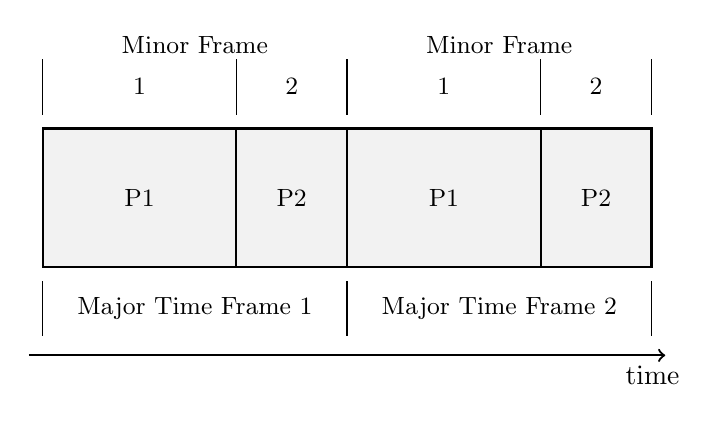
\begin{tikzpicture}[scale=1]
		{
			\def\boxh{50pt}
			\def\lineh{20pt}
			\def\off{110pt}
			\def\nodestyle{node[pos=0.5,font=\small]}
			\foreach \o in {0,...,1}
			{
				\pgfmathtruncatemacro{\mtlabel}{\o + 1}

				\path (\off*\o+00pt, \boxh+\lineh+10pt) -- ++(\off, 0pt) \nodestyle {Minor Frame};
				\draw (\off*\o+00pt, \boxh+5pt) -- ++(0pt, \lineh);
				\path (\off*\o+00pt, \boxh+5pt) -- ++(70pt, \lineh) \nodestyle
					(min\o) {1};

				\draw (\off*\o+70pt, \boxh+5pt) -- ++(0pt, \lineh);
				\path (\off*\o+70pt, \boxh+5pt) -- ++(40pt, \lineh)
				\nodestyle (min\o) {2};

				\draw (\off*\o+\off, \boxh+5pt) -- ++(0pt, \lineh);

				\draw[thick, fill=gray, fill opacity=0.10, text opacity=1.0] (\off*\o+00pt,0pt) rectangle +(70pt,\boxh) \nodestyle {P1};
				\draw[thick, fill=gray, fill opacity=0.10, text opacity=1.0] (\off*\o+70pt,0pt) rectangle +(40pt,\boxh) \nodestyle {P2};

				\path (\off*\o+0pt,-\lineh-5pt) -- ++(\off, \lineh) \nodestyle (mt\o) {Major Time
				Frame \mtlabel};
				\draw (\off*\o+0pt,-\lineh-5pt) -- ++(0pt, \lineh);
				\draw (\off*\o+\off,-\lineh-5pt) -- ++(0pt, \lineh);
			}
			\draw[thick, ->] (-5pt,-\lineh-12pt) -- (2*\off+5pt, -\lineh-12pt)
			node[pos=0.98,below] {time};
		}
	\end{tikzpicture}
	\caption{Partition scheduling}
	\label{figure:partition_scheduling}
\end{figure}

ARINC 653 partition scheduler and process scheduler handle tasks differently. Process scheduler
needs to handle tasks depending whether the task is periodic or aperiodic. Meanwhile, partition
scheduler works as described regardless of whether the task is periodic or aperiodic. For
example, \figurename ~\ref{figure:partition_scheduling} illustrates one case in which we have 2
partitions to be scheduled. Each partition have their own minor frame which spans for a
determined time. After the first major time frame executed, the scheduler then do the next major
time frame. For aperiodic tasks, it should be sufficient to just make sure the major time frame
is less than the deadline. This makes sure that the partition with this task would be selected
at least once to do the task. For periodic tasks, the scheduler need to be configured properly.
\figurename ~\ref{figure:periodic_task_scheduling} illustrates periodic tasks scheduling.
Suppose that we have 3 domains with minor frames of 5, 6, 10 ms and the worst case running times
of these partitions are 1 ms, 2 ms, and 3 ms respectively. The major frame should be set to the
least common multiples of these minor frames, which is 30 ms, so that the deadline for each of
these partitions can be met.

\begin{figure}
	\def\run{black}
	\centering
	\subfloat{
		\begin{tabular}{|r|c|c|c|}
			\hline
			ms & P1 & P2 & P3 \\ \hline
			0&&&\cellcolor{\run}\\ \hline
			1&&&\cellcolor{\run}\\ \hline
			2&&&\cellcolor{\run}\\ \hline
			3&\cellcolor{\run}&&\\ \hline
			4&&\cellcolor{\run}&\\ \hline
			5&&\cellcolor{\run}&\\ \hline
			6&&&\\ \hline
			7&\cellcolor{\run}&&\\ \hline
			8&&\cellcolor{\run}&\\ \hline
			9&&\cellcolor{\run}&\\ \hline
			10&&&\cellcolor{\run}\\ \hline
			11&&&\cellcolor{\run}\\ \hline
			12&&&\cellcolor{\run}\\ \hline
			13&\cellcolor{\run}&&\\ \hline
			14&&\cellcolor{\run}&\\ \hline
		\end{tabular}
	}
	\subfloat{
		\begin{tabular}{|r|c|c|c|}
			\hline
			ms & P1 & P2 & P3 \\ \hline
			15&&\cellcolor{\run}&\\ \hline
			16&&&\\ \hline
			17&\cellcolor{\run}&&\\ \hline
			18&&\cellcolor{\run}&\\ \hline
			19&&\cellcolor{\run}&\\ \hline
			20&&&\cellcolor{\run}\\ \hline
			21&&&\cellcolor{\run}\\ \hline
			22&&&\cellcolor{\run}\\ \hline
			23&\cellcolor{\run}&&\\ \hline
			24&&\cellcolor{\run}&\\ \hline
			25&&\cellcolor{\run}&\\ \hline
			26&&&\\ \hline
			27&\cellcolor{\run}&&\\ \hline
			28&&&\\ \hline
			29&&&\\ \hline
		\end{tabular}
	}
	\caption{Periodic tasks scheduling}
	\label{figure:periodic_task_scheduling}
\end{figure}

\subsection{ARLX ARINC 653 Scheduler}
ARINC 653 scheduler on ARLX selects one of the runnable partition from a fixed partition list
given by hypercall \cite{VanderLeest2010}. The list consists of partition, its supposed run
time, and assigned VCPU identification to execute the domain. The scheduler then selects the
partition in round-robin fashion. It assigns the corresponding VCPU responsible for the
partition to run if the VCPU is awake and runnable. The order of partitions to be selected is
fixed and is the same as the partition list.

There are some differences between standard ARINC 653 scheduler and ARLX.

\begin{itemize}
	\item In ARLX, the schedule is configured manually with hypercalls instead of
		being generated by time-based activation. It is the engineer responsibility to
		determine how much CPU time being allocated to each partition.

	\item ARLX only modifies Xen hypervisor code and it only concerns with the hypervisor
		aspects, so it only provides partition scheduler that is compliant to ARINC 653
		specification. Process scheduling for real-time processes inside of each
		partition are handled by operating system on that partition.

	\item Multicore support for partition scheduling is not yet implemented, so we only deal
		with uniprocessor architecture.
\end{itemize}

\section{Improving Service Reliability}

The problem with faulty partition is that the service it provides will cease to work and/or give
incorrect result. In avionics, this could lead to incorrect calculation of control systems, thus
significantly increases safety-risk for people and/or environment involved. We assume that there
is one-to-one relationship between service and partition. The simplest way to bring back the
service is by restarting the faulty partition. In general cases, there is no way to know whether
restarting faulty partition could bring back said service as the cause of fault could be
persistent.

To improve service reliability in real-time systems, one solution is to have the scheduler to be
fault-tolerant \cite{Campbell1986} \cite{Han2003} \cite{Shin2008}. A study shows that a
hierarchical scheduler like ARINC 653 scheduler, which has at least two levels of scheduling,
can be made fault-tolerant with primary-backup scheme \cite{Jin2013}. When a partition
experienced failure, the scheduler can keeps the service running by having backup partition
running in place of the faulty primary partition. Common primary-backup schemes make sure that
each partition have replicas that is identical service-wise to the primary partition before
being operational. When said partition experienced a failure, one of its replicas could take
over its place and provide the same service. While this scheme can seamlessly handle persistent
failure on partitions, identical partitions means the exact same failure in primary are bound to
happen in replicas.

For primary-backup scheme on partition scheduler to work indefinitely, replica partitions should
not be identical to their corresponding primary partition. We could think of replicas as
fail-safe mechanism of corresponding primary. This could be achieved by having more mature
application and environments in replicas. We assume that mature version of the application
provide identical service to current version of the application, although it might lack some
non-essential features or optimizations. For applications that do not support backward
compatibility, having flexibility in choosing applications that resides in replicas means we
still have the option to use identical replicas.

\section{Primary-Backup ARINC 653 Scheduler}

In this section, we will look at some implementation details which make primary-backup scheme on
ARINC 653 scheduler possible. Then we will do availability testing for the resulting scheduler.

\subsection{Partition Information}

For the scheduler to know whether a partition should run or not, it needs to know if that
partition is currently okay to run. We will call such information as partition status. The
scheduler also needs information about the service provided in a partition, so the scheduler
does not confuse which primary partition that each backup partition corresponds to. This can be
done by giving service identification and make sure each partition keep its service
identification. Since we already assume one-to-one relationship between service and partition,
service identification can use partition identification, which already provided by default in
ARLX.

Each partition should keep track of their own status and service identification that it
provides. To let the scheduler know current partition status and service identification, we need
a way to update partition status. This could be done through calling hypercalls from each
partition or intelligent health monitoring. We implement the hypercall method, as it is easy to
implement and offer flexibility for configuration. From base ARINC 653 scheduler on ARLX, we
implement partition information in domain private data. We also implement scheduler hypercalls
on domain-specific context.

\subsection{The Scheduling Strategy}

To keep the scheduling deterministic, we need to make sure that the algorithm will not depend on
external sources. The input of the scheduling algorithm is partition information which already
discussed in the last part. The scheduler selects one of the runnable partition such that its
status is healthy and there are no partitions that have provided the service corresponding to
its service identification. When the scheduler scans the schedule list, we extend it to also
check whether the partition satisfies said conditions.

It is trivial to check whether the partition is healthy. To check whether the service it
provides have been provided before, we need a flag for possible service identification value.
The flag is initialized to zero for all services at first. When a partition already exhausted
its quantum, the scheduler then toggle the flag for the corresponding service. This is feasible
without changing the required space complexity for the scheduler. Since service identification
value corresponds to partition identification, thus its value is incremental from $1$ to $N$
with $N$ is the number of partitions available. Thus, the extra space in the scheduler we need
for the flag is linear to the number of partitions, which is the same as the schedule list
itself.

\begin{figure}[ht]
	\centering
	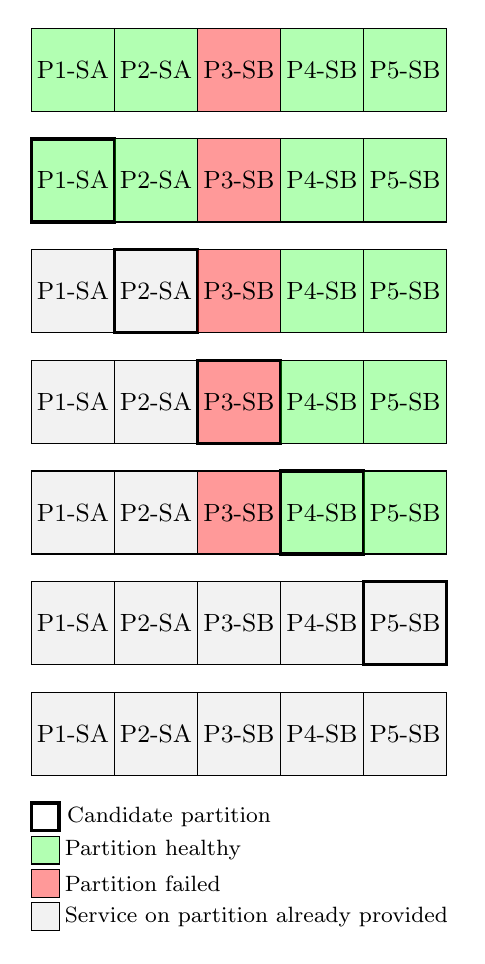
\begin{tikzpicture}[
		partition-done/.style={fill=gray, fill opacity=0.10, text opacity=1.0},
		partition-healthy/.style={fill=green, fill opacity=0.30, text
		opacity=1.0},
		partition-failed/.style={fill=red, fill opacity=0.40, text opacity=1.0},
		candidate/.style={very thick},
		]

		\def\boxs{30pt}
		\def\legends{10pt}
		\def\off{10pt}
		\def\loff{2pt}
		\def\shape{rectangle +(\boxs,\boxs)}
		\def\partnode{node[pos=0.5,font=\small]}
		\def\lshape{rectangle +(\legends,\legends)}
		\newcommand\lnode[1]{node[pos=0.5,align=right,label={[anchor=west,font=\footnotesize]right:#1}] {}}

		\draw[partition-healthy]           (0*\boxs,{0*(-\boxs-\off)}) \shape \partnode {P1-SA};
		\draw[partition-healthy]           (1*\boxs,{0*(-\boxs-\off)}) \shape \partnode {P2-SA};
		\draw[partition-failed]            (2*\boxs,{0*(-\boxs-\off)}) \shape \partnode {P3-SB};
		\draw[partition-healthy]           (3*\boxs,{0*(-\boxs-\off)}) \shape \partnode {P4-SB};
		\draw[partition-healthy]           (4*\boxs,{0*(-\boxs-\off)}) \shape \partnode {P5-SB};

		\draw[partition-healthy,candidate] (0*\boxs,{1*(-\boxs-\off)}) \shape \partnode {P1-SA};
		\draw[partition-healthy]           (1*\boxs,{1*(-\boxs-\off)}) \shape \partnode {P2-SA};
		\draw[partition-failed]            (2*\boxs,{1*(-\boxs-\off)}) \shape \partnode {P3-SB};
		\draw[partition-healthy]           (3*\boxs,{1*(-\boxs-\off)}) \shape \partnode {P4-SB};
		\draw[partition-healthy]           (4*\boxs,{1*(-\boxs-\off)}) \shape \partnode {P5-SB};

		\draw[partition-done]              (0*\boxs,{2*(-\boxs-\off)}) \shape \partnode {P1-SA};
		\draw[partition-done,candidate]    (1*\boxs,{2*(-\boxs-\off)}) \shape \partnode {P2-SA};
		\draw[partition-failed]            (2*\boxs,{2*(-\boxs-\off)}) \shape \partnode {P3-SB};
		\draw[partition-healthy]           (3*\boxs,{2*(-\boxs-\off)}) \shape \partnode {P4-SB};
		\draw[partition-healthy]           (4*\boxs,{2*(-\boxs-\off)}) \shape \partnode {P5-SB};

		\draw[partition-done]              (0*\boxs,{3*(-\boxs-\off)}) \shape \partnode {P1-SA};
		\draw[partition-done]              (1*\boxs,{3*(-\boxs-\off)}) \shape \partnode {P2-SA};
		\draw[partition-failed,candidate]  (2*\boxs,{3*(-\boxs-\off)}) \shape \partnode {P3-SB};
		\draw[partition-healthy]           (3*\boxs,{3*(-\boxs-\off)}) \shape \partnode {P4-SB};
		\draw[partition-healthy]           (4*\boxs,{3*(-\boxs-\off)}) \shape \partnode {P5-SB};

		\draw[partition-done]              (0*\boxs,{4*(-\boxs-\off)}) \shape \partnode {P1-SA};
		\draw[partition-done]              (1*\boxs,{4*(-\boxs-\off)}) \shape \partnode {P2-SA};
		\draw[partition-failed]            (2*\boxs,{4*(-\boxs-\off)}) \shape \partnode {P3-SB};
		\draw[partition-healthy,candidate] (3*\boxs,{4*(-\boxs-\off)}) \shape \partnode {P4-SB};
		\draw[partition-healthy]           (4*\boxs,{4*(-\boxs-\off)}) \shape \partnode {P5-SB};

		\draw[partition-done]              (0*\boxs,{5*(-\boxs-\off)}) \shape \partnode {P1-SA};
		\draw[partition-done]              (1*\boxs,{5*(-\boxs-\off)}) \shape \partnode {P2-SA};
		\draw[partition-done]              (2*\boxs,{5*(-\boxs-\off)}) \shape \partnode {P3-SB};
		\draw[partition-done]              (3*\boxs,{5*(-\boxs-\off)}) \shape \partnode {P4-SB};
		\draw[partition-done,candidate]    (4*\boxs,{5*(-\boxs-\off)}) \shape \partnode {P5-SB};

		\draw[partition-done]              (0*\boxs,{6*(-\boxs-\off)}) \shape \partnode {P1-SA};
		\draw[partition-done]              (1*\boxs,{6*(-\boxs-\off)}) \shape \partnode {P2-SA};
		\draw[partition-done]              (2*\boxs,{6*(-\boxs-\off)}) \shape \partnode {P3-SB};
		\draw[partition-done]              (3*\boxs,{6*(-\boxs-\off)}) \shape \partnode {P4-SB};
		\draw[partition-done]              (4*\boxs,{6*(-\boxs-\off)}) \shape \partnode {P5-SB};

		% legends
		\draw[candidate] (0pt,{6*(-\boxs-\off)-0*(\legends+\loff)-\legends-\off}) \lshape
		\lnode{Candidate partition};

		\draw[partition-healthy]
		(0pt,{6*(-\boxs-\off)-1*(\legends+\loff)-\legends-\off}) \lshape
		\lnode{Partition healthy};

		\draw[partition-failed]
		(0pt,{6*(-\boxs-\off)-2*(\legends+\loff)-\legends-\off}) \lshape
		\lnode{Partition failed};

		\draw[partition-done]
		(0pt,{6*(-\boxs-\off)-3*(\legends+\loff)-\legends-\off}) \lshape
		\lnode{Service on partition already provided};

	\end{tikzpicture}
	\caption{Primary-backup scheduling}
	\label{figure:pb_scheduling}
\end{figure}

We illustrate how primary-backup ARINC 653 scheduler work in \figurename
~\ref{figure:pb_scheduling}. The scheduler has a list of partitions to be scheduled. These
partition each have current status (healthy/failed) and service identification. When the
scheduler should determine whether the candidate partition will be given CPU time or not, the
scheduler will check if the partition is healthy and the service corresponding to service
identification is not provided yet. In \figurename ~\ref{figure:pb_scheduling}, the partition
label has the format P$X$-S$Y$, which means partition $X$ will provide service $Y$ if given CPU
time. On a particular major time frame, the algorithm will work as follows:

\begin{itemize}

	\item On partition P1, the partition is healthy and service $A$ is not yet provided, so
		the partition is given the CPU time,

	\item Partition P2 however, is not given the CPU time, as when partition P1 exhausted
		its quantum, service $A$ is already provided.

	\item For partition P3, the corresponding service is not yet provided, but the partition
		is currently failed, thus is not given the CPU time.

	\item Partition P4 is healthy, and since partition P3 is not given the CPU time, the
		corresponding service has not yet provided. Since all condition is satisfied,
		partition P4 is given CPU time.

	\item Partition P5 is not given the CPU time, as the corresponding service, service $B$
		is already provided by partition P4.

\end{itemize}

At the end of the major time frame, this algorithm ensures that given a service will be provided
if there is at least one partition providing the service that is healthy. The algorithm will
restart this process if current major time frame is elapsed. This whole process will be done
indefinitely.

\subsection{Reliability Testing}

To measure whether the proposed scheduler improve system reliability, the system is to be tested
for its reliability while using the scheduler. The primary goal of this reliability testing is
to measure mean time to failure for the system. We can assume that the system will always fail
when any service is failed and the service is the most unreliable component of the system, thus
the system mean time to failure is the same as the minimum mean time to failure of all services.
Since we want to prolong the system mean time to failure, we want to maximize the mean time to
failure for all services. The testing result can also be used to validate whether the algorithm
works as intended.

Reliability testing is done by checking whether each partition can successfully pass heartbeat
check. The partition is said to be successfully pass heartbeat check when it sends heartbeat if
and only if the partition satisfies the running condition. One simple way to do this is by
creating a testing framework with server-client architecture. Each partition is a client, and we
can have any machine as the server, as long as all the partitions is connected to the server
machine by any means. Each partition then sends heartbeat with its service identification and
partition identification to the server on a fixed interval. The server makes sure that each
service is provided, while noting which partition provides the service.

We tested the primary-backup ARINC 653 scheduler by having five partitions, named as P1 to P5.
The first two partitions (P1 and P2) provide service $A$ and the last three partitions (P3, P4,
and P5) provide service $B$. The testing scenarios on these partitions, including the expected
outcome, are as follows:

\begin{enumerate}
	\item Initially, all five partitions are healthy. In this scenario, the scheduler are
		supposed to selects partition P1 and partition P3.

	\item Partition P3 experienced a failure. In this scenario, the scheduler are supposed
		to selects partition P1 and partition P4. This scenario is exactly the same as
		illustrated in \figurename ~\ref{figure:pb_scheduling}.

	\item Partition P2, P3, and P5 then experienced a failure. In this scenario, the
		scheduler are supposed to selects partition P1 and partition P5. This scenario is
		done to test the scheduler behavior. The scheduler should still choose a
		candidate which meets the running conddition, even when there are backup
		partitions, which to be scheduled later than the candidate experienced a
		failure. 
\end{enumerate}

In the first scenario, when all partitions are healthy, the server receive service $A$ from
partition P1 and service P2 from partition P3. For the second scenario, the server receives
heartbeat from partition P1 for service $A$ and from partition P4 for service $B$. This means
the service still functioning correctly even when the original partition which provides the
service experiencing a failure. On the third scenario, the server still receives heartbeat for
service $A$ from partition P1 and service $B$ from partition P4. This means failured experienced
by backup partitions later than the supposed selected partitions do not affect scheduler
selection.

In all of these scenarios, all the service required is provided, even though partitions can
still experience failures as base ARINC 653 scheduler. This means, while this scheme does not
increases the mean time to failure for each partition, it does increases mean time to failure
for each service. 

\section{Conclusion}

In this paper, we proposed a way to increases the reliability of ARINC 653 operating systems by
using primary-backup scheme on ARINC 653 partition scheduler. The scheduler works by giving CPU
time to candidate partition only when it is currently healthy and the corresponding service has
not provided yet. In order to let the scheduler know partition status, we define a new hypercall
to modify information associated to a partition. Using primary-backup scheme on ARINC 653
scheduler increases the reliability for each service and thus prolong the mean time to failure
for any service. Since we assume that services reliability is the most unreliable component on the
system, this means the proposed scheduler also increases the whole system reliability.

While the result of the reliability testing is already good, the testing is done without regards
of processes' deadline inside of each partition. We intend to do some improvement on the testing
method so it also considers the deadline of each process inside of each partition. Doing so will
make the result more relevant to the actual use case of the system. We also plan to have
another type of test to measure performance difference caused by the overhead of the scheduler
and analyze the effect of the difference on the system.

As the paper proposed a new scheduler, there are some issues which need to be solved such as:

\begin{itemize}

	\item \textit{Space redundancy minimization}: Having backup partitions require extra
		space linear to the average redundancy rate of primary partitions for the
		system. On the assumption that the mean time to failure for each service to be
		reasonably long, we might be able to reduce system required space in overall at
		the cost of performance on rare events.

	\item \textit{Automatic partition failure detection}: Telling the scheduler whether the
		service on a partition is healthy or not can already be done by means of
		hypercalls. This cannot be done if the environment on said partition does not
		functions properly, which can be caused by transient or inherent problems. The
		hypervisor must be able detect such cases automatically so the scheduler could
		properly select one of the backup partitions.

	\item \textit{Multicore support}: Some of the inherent problems that could happen is
		failure of the CPU core which the partition is supposed to run.
		Having some other cores could help the scheduler schedule the backup partitions
		on different core than the primary to keep the service running.

		\newpage

	\item \textit{Automatic schedule list generator}: It is up to the engineer to provide a
		schedule list which satisfies the deadline and runtime constraints. Since the
		schedule list might need to be adjusted when a partition failure occurs, the
		scheduler list should still satisfies the deadline and runtime constraints on
		any possible partitions state. This proves to be a daunting task for the
		engineer since there will be many cases (up to $2^N$ possible cases, $N$ is the
		number of partitions).

\end{itemize}

% conference papers do not normally have an appendix



% use section* for acknowledgment
\ifCLASSOPTIONcompsoc
  % The Computer Society usually uses the plural form
  % \section*{Acknowledgments}
\else
  % regular IEEE prefers the singular form
  % \section*{Acknowledgment}
\fi


% The authors would like to thank...





% trigger a \newpage just before the given reference
% number - used to balance the columns on the last page
% adjust value as needed - may need to be readjusted if
% the document is modified later
%\IEEEtriggeratref{8}
% The "triggered" command can be changed if desired:
%\IEEEtriggercmd{\enlargethispage{-5in}}

% references section

% can use a bibliography generated by BibTeX as a .bbl file
% BibTeX documentation can be easily obtained at:
% http://mirror.ctan.org/biblio/bibtex/contrib/doc/
% The IEEEtran BibTeX style support page is at:
% http://www.michaelshell.org/tex/ieeetran/bibtex/
%\bibliographystyle{IEEEtran}
% argument is your BibTeX string definitions and bibliography database(s)
%\bibliography{IEEEabrv,../bib/paper}
%
% <OR> manually copy in the resultant .bbl file
% set second argument of \begin to the number of references
% (used to reserve space for the reference number labels box)
% \begin{thebibliography}{1}

\begin{thebibliography}{1}

\bibitem{Rushby2000}
John Rushby.
\newblock {Partitioning in avionics architectures: requirements, mechanisms and
  assurance}.
\newblock {\em Work}, (March):67, 2000.

\bibitem{AirlinesElectronicEngineeringCommittee2012}
{Airlines Electronic Engineering Committee}.
\newblock {653P1-3 Avionics Application Software Standard Interface Part 1 -
  Required Services}.
\newblock {\em Arinc 653}, page~85, 2012.

\bibitem{Campbell1986}
Arthur~L. Liestman and Roy~H. Campbell.
\newblock {A Fault-Tolerant Scheduling Problem}.
\newblock {\em IEEE Transactions on Software Engineering},
  SE-12(11):1089--1095, 1986.

\bibitem{Han2003}
Ching~Chih Han, Kang~G. Shin, and Jian Wu.
\newblock {A fault-tolerant scheduling algorithm for real-time periodic tasks
  with possible software faults}.
\newblock {\em IEEE Transactions on Computers}, 52(3):362--372, 2003.

\bibitem{Shin2008}
Insik Shin and Insup Lee.
\newblock {Compositional real-time scheduling framework with periodic model}.
\newblock {\em ACM Transactions on Embedded Computing Systems}, 7(3):1--39,
  2008.

\bibitem{Jin2013}
Hyun-Wook Jin.
\newblock {Fault-tolerant hierarchical real-time scheduling with backup
  partitions on single processor}.
\newblock {\em ACM SIGBED Review}, 10(4):25--28, 2013.

\bibitem{VanderLeest2010}
Steven~H. VanderLeest.
\newblock {ARINC 653 hypervisor}.
\newblock In {\em AIAA/IEEE Digital Avionics Systems Conference - Proceedings},
  2010.

\end{thebibliography}

% \bibliographystyle{plain}
% \bibliography{refs}

\end{document}

% vim: tw=96
